\documentclass[conference]{IEEEtran}
\IEEEoverridecommandlockouts
% The preceding line is only needed to identify funding in the first footnote. If that is unneeded, please comment it out.
\usepackage[english]{babel}
\usepackage{cite}
\usepackage{amsmath,amssymb,amsfonts,mathtools}
\usepackage{algorithmic}
\usepackage{graphicx}
\usepackage{textcomp}
\usepackage[dvipsnames]{xcolor}
\def\BibTeX{{\rm B\kern-.05em{\sc i\kern-.025em b}\kern-.08em
    T\kern-.1667em\lower.7ex\hbox{E}\kern-.125emX}}
\usepackage{listings}
\usepackage{tabularx}
\usepackage{booktabs}
\usepackage{siunitx}
\usepackage{float}
\usepackage{caption}

\definecolor{codegreen}{rgb}{0,0.6,0}
\definecolor{codegray}{rgb}{0.5,0.5,0.5}
\definecolor{codepurple}{rgb}{0.58,0,0.82}
\definecolor{backcolour}{rgb}{0.95,0.95,0.95}
\renewcommand{\lstlistingname}{Code}% Listing -> Algorithm
\renewcommand{\lstlistlistingname}{List of \lstlistingname s}% List of Listings -> List of Algorithms
\lstdefinestyle{mystyle}{
    backgroundcolor=\color{backcolour},
    commentstyle=\color{codegreen},
    keywordstyle=\color{magenta},
    numberstyle=\tiny\color{codegray},
    stringstyle=\color{codepurple},
    basicstyle=\ttfamily\footnotesize,
    breakatwhitespace=false,
    breaklines=true,
    captionpos=b,
    keepspaces=true,
    numbers=left,
    numbersep=3pt,
    showspaces=false,
    showstringspaces=false,
    showtabs=false,
    tabsize=3
}
\lstset{style=mystyle}

\usepackage{hyperref}
\hypersetup{
    pdftex,
    pdftitle={Versuch GM-Klein},
    pdfsubject={Versuch GM-Klein},
    pdfauthor=AJC,
    colorlinks,
    citecolor=black,
    filecolor=black,
    linkcolor=black,
    urlcolor=black
}

\author{
    \IEEEauthorblockN{
        \textsc{Ayham Alhalaibi}
    }
    \and
    \IEEEauthorblockN{
        \textsc{Julia Blechle}
    }
    \and
    \IEEEauthorblockN{
        \textsc{Clara Huber}
    }
}

\begin{document}

\title{
    \centering
    
\includegraphics[width=0.5\textwidth]{../OTHR_OTHR_Logo.pdf}\\
    \textsc{DC machine - small} \\
}

\maketitle

\begin{abstract}

    In this experiment the behavior of a small DC machine was studied in
    different operating modes. The machine was operated in three different
    modes: \textit{Idle}, \textit{loaded generator}, and \textit{loaded motor}.
    The test machine was connected to a variable power supply
    0\si{V}\dots12\si{V} and a DC generator was loaded with 5 resistors in
    parallel, which can be switched on and off with a switch box. Both machines
    had a built-in meters for the armature current and voltage also for the
    number of rotations.

\end{abstract}

\section{Idle mode experiment}
\subsection{Electric motor force}

The induced voltage in the generator is called electric motor force
($\mathrm{EMK}$).

To examine the relation between the electric motor force and the rotations $n$,
the machine is operated without load and the motor voltage and current as well
as $\mathrm{EMK}$ which is induced in the generator can be measured.

For this experiment the initial 5000rpm will be reduced by 1000rpm each
time. At 5000rpm the motor has its maximum voltage $U_A = 11.94V$.

The machine constant $c$ and the magnetic flux $\Phi_E$ are experimentally
determined (different for each machine).

\begin{equation} \label{eq:machine_const}
    c \cdot \Phi_E = \frac{U_q}{n} = \frac{8.8\si{V}}{4000/60\si{s}} = 0.132\si{Vs}
\end{equation}

The arithmetic mean is calculated using the following equation:

\begin{equation}
    \frac{1}{5}\sum\limits_{k = 1}^{5} c \cdot \Phi_E = \frac{0.6621Vs}{5} = 0.13242Vs
\end{equation}

\begin{figure}[htbp]
    \centering
    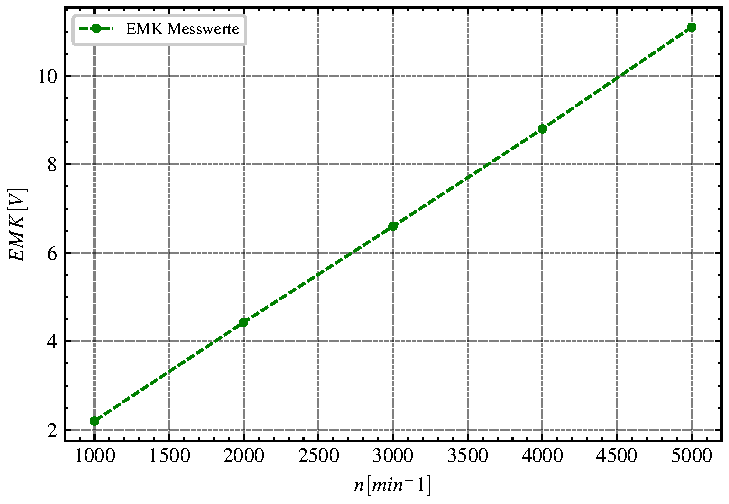
\includegraphics[width=\columnwidth]{plots/4.1_Leerlaufversuch.pdf}
    \caption{Idle Mode}
    \label{fig:emk_n}
\end{figure}

\begin{table}[htbp]
    \centering
    \begin{tabularx}{\columnwidth}{XXXXX}
        \toprule
        $n[min^{-1}]$ & $EMK[V]$ & $U_A[V]$ & $I_A[A]$ & $c\cdot\varphi_E[Vs]$ \\
        \midrule
        5000          & 11.10    & 11.94    & 0.420    & 0.1332                \\
        4000          & 8.80     & 9.61     & 0.390    & 0.1320                \\
        3000          & 6.60     & 7.30     & 0.357    & 0.1320                \\
        2000          & 4.43     & 5.00     & 0.327    & 0.1329                \\
        1000          & 2.20     & 2.68     & 0.276    & 0.1320                \\
        \bottomrule
    \end{tabularx}
    \caption{Idle Mode}
    \label{tab:idle_mode}
\end{table}



In the figure \ref{fig:emk_n} the relation between the electric motor force
$EMK$ and the number of rotations $n$ is shown. The relation is linear and they
are directly proportional.


\section{loaded generator mode}

In the generator mode the generator machine is powering the motor. The
rotations are set at 4000rpm.

In the previous experiment the motor voltage was measured at 4000rpm.
Throughout this experiment this voltage will be kept constant at $U_q(4000rpm)
    = 8.8V$. The load resistors are getting connected into the circuit one by one.


\begin{figure}[htbp]
    \centering
    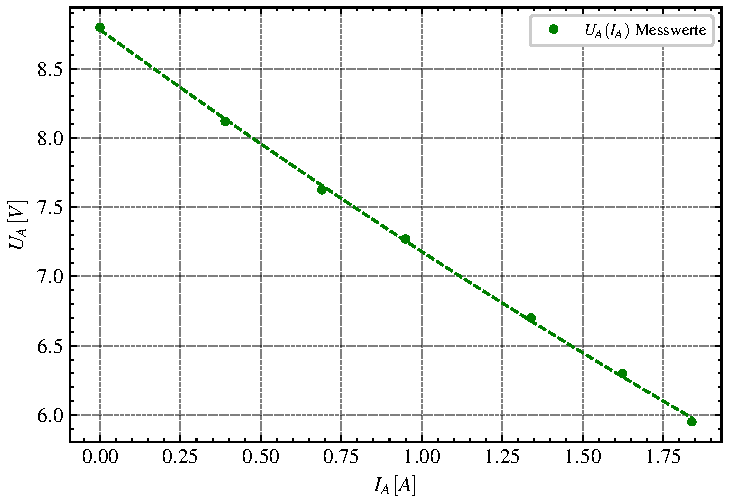
\includegraphics[width=\columnwidth]{plots/4.2_Belasteter_Generator_4000.pdf}
    \caption{loaded generator mode}
    \label{fig:load_generator_mode}
\end{figure}

To determine the resistance $R_A$ of the generator the potential over said
resistor as well as the current running through it are needed.

\begin{equation} \label{eq:R_A_resistance}
    R_A = \frac{U_{RA}}{I_A} = \frac{U_A - U_q}{I_A}
\end{equation}

With the arithmetic mean
\begin{equation}
    \frac{1}{6} \sum\limits_{k = 1}^{6} c \cdot R_A = 1.62 \Omega
\end{equation}


\section{loaded motor mode}
In the loaded motor mode the voltage $U_A$ is kept constant, first at 9V later
at 12V, and is loaded through the generator with the load resistors (S1 - S5).

The relation between the armature voltage and the rotor rotations is given
through the machine constant $c$ as described in \ref{eq:rotor_rotations}.

\begin{equation} \label{eq:rotor_rotations}
    n_0 = \frac{U_A}{c \cdot \Phi_E}
\end{equation}

And the correlation between the inner torque and armature current:

\begin{equation} \label{eq:inner_tourque}
    M_i = \frac{c \cdot \Phi_E \cdot I_A}{2 \pi}
\end{equation}

% From the correlation in \ref{eq:inner_tourque}

Between the inner and the measured torque, Power is lost through Copper
$P_\mathrm{Cu}$ and friction $ P_\text{fric}$.

To measure the Torque of the motor a metal arm (10cm) fixed to its bearing and
a small scale are used. With the following equation the torque is calculated
for each of the resistor combinations:

\begin{equation}
    M = \text{Weight} \cdot \mathrm{g} \cdot \text{length} \qquad g=9.81
    \si{m}^2 \quad l=10 \si{cm}
    \label{eq:tourqe_weight_length}
\end{equation}


\begin{table}[htbp]
   \centering
   \begin{tabularx}{\columnwidth}{XXXXXXX}
      \toprule
      Switches    & $n [min^{-1}]$ & $I_A [A]$ & Weight$[g]$ & $M[m\, Nm]$ \\
      \midrule
      All Open    & 3766           & 0.386     & 8.08        & 7.924       \\
      S1          & 3548           & 0.724     & 9.29        & 9.110       \\
      S2          & 3385           & 0.958     & 10.75       & 10.54       \\
      S1+S2       & 3261           & 1.146     & 11.53       & 11.31       \\
      S1+S2+S3    & 3080           & 1.400     & 13.75       & 13.48       \\
      S1+S2+S3+S4 & 2962           & 1.565     & 15.15       & 14.86       \\
      All Closed  & 2868           & 1.680     & 16.70       & 16.38       \\
      \bottomrule
   \end{tabularx}
   \caption{Belasteter Motor $U_A=9V$}
\end{table}

\begin{table}[htbp]
   \centering
   \begin{tabularx}{\columnwidth}{XXXXXXX}
      \toprule
      Switches    & $n [min^{-1}]$ & $I_A ,[A]$ & Weight $[g]$ & $M [m\,Nm]$ \\
      \midrule
      All Open    & 5100           & 0.41       & 8.06         & 7.90        \\
      S1          & 4760           & 0.87       & 8.66         & 8.49        \\
      S2          & 4563           & 1.20       & 9.22         & 9.04        \\
      S1+S2       & 4390           & 1.44       & 10.15        & 9.95        \\
      S1+S2+S3    & 4150           & 178.00     & 12.48        & 12.24       \\
      S1+S2+S3+S4 & 3980           & 2.02       & 14.60        & 14.32       \\
      All Closed  & 3910           & 2.20       & 16.93        & 16.60       \\
      \bottomrule
   \end{tabularx}
   \caption{Loaded motor mode - $U_A=12V$}
\end{table}


The plot \ref{fig:loaded_motor_mode} shows the torque of the motor driven with
two different voltages $U_A$. It also displays the linear correlation between the
torque and rotations.

After disregarding the Copper and friction and assuming linearity the plot
\ref{fig:loaded_motor_mode} perfectly demonstrates how changing the voltage
results in a shift of the torque curve on the n-axis and showing the direct
proportionality between the voltage and the rotations. Also see equation
\ref{eq:rotor_rotations}.

\begin{figure}[htbp]
    \centering
    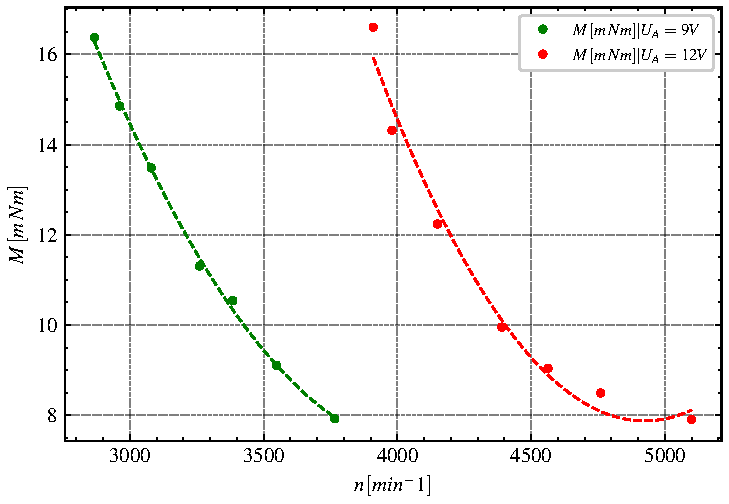
\includegraphics[width=\columnwidth]{plots/4.3_Belasteter_Motor_UA9V_12V.pdf}
    \caption{loaded motor mode}
    \label{fig:loaded_motor_mode}
\end{figure}


\end{document}
